% ----- formatovani dokumentu -----------------------------------------------
\documentclass[12pt,a4paper,titlepage,final]{report}
\usepackage[utf8]{inputenc}
\usepackage[T1, IL2]{fontenc}
\usepackage{graphicx}
\usepackage{epstopdf}
\usepackage[margin=2cm]{caption}
\usepackage[top=3cm, left=2cm, right=2cm, text={17cm, 24cm}, ignorefoot]{geometry}
\usepackage{color}
\usepackage{url}
\usepackage{setspace}
\singlespacing
\usepackage[square, numbers]{natbib} 
\usepackage{float}
\pagestyle{plain}
\pagenumbering{arabic}
\setcounter{page}{1}
\setcounter{secnumdepth}{-1}
\setlength{\parindent}{1cm}	
\usepackage{natbib}
\usepackage{amsmath}
\usepackage{tocloft}
\usepackage{esvect}
\usepackage{amssymb}
\usepackage{gensymb}
\usepackage{subcaption}
\usepackage[algoruled,boxed,lined,longend]{algorithm2e}
\usepackage{mathtools}
\usepackage{listings}

\DeclareMathOperator{\dis}{d}

  \newenvironment{czechalgorithm}[1][htb]
  {\renewcommand{\algorithmcfname}{Algoritmus}% Update algorithm name
   \begin{algorithm}[#1]%
  }{\end{algorithm}}

% ----- vyberte jazyk -------------------------------------------------------
\usepackage[english,czech]{babel}
%\usepackage[english]{babel}

% ----- dopiste titulky -----------------------------------------------------
\newcommand\Course{Kódování a komprese dat}
\newcommand\WorkTitle{Komprese obrazových dat s využitím adaptivního Huffmanova kódování}
\newcommand\Author{Petr Flajšingr}
\newcommand\AuthorEmail{xflajs00@stud.fit.vutbr.cz}
\newcommand\Faculty{Fakulta Informačních Technologií}
\newcommand\School{Vysoké Učení Technické v Brně}

\usepackage[
pdftitle={\WorkTitle},
pdfauthor={\Author}
bookmarks=true,
colorlinks=true,
breaklinks=true,
urlcolor=blue,
citecolor=blue,
linkcolor=blue,
unicode=true,
]
{hyperref}


% ----- titulni strana ------------------------------------------------------

\begin{document}
	\begin{titlepage}
	\begin{center}
		
\includegraphics[height=5cm]{images/logo.eps}
	\end{center}
	\vfill
	\begin{center}
		\begin{Large}
			\Course\\
		\end{Large}
		\bigskip
		\begin{Huge}
			\WorkTitle\\
		\end{Huge}
	\end{center}
	\vfill
	\begin{center}
		\begin{large}
			\today
		\end{large}
	\end{center}
	\vfill
	\begin{flushleft}
		\begin{large}
			\begin{tabular}{lll}
				Autoři: & \Author, & \url{\AuthorEmail} \\
				& \Faculty \\
				& \School \\
			\end{tabular}
		\end{large}
	\end{flushleft}
\end{titlepage}		

\section{Úvod}
Cílem projektu je implementace programu pro kompresi obrázků v raw formátu za využití adaptivního Huffmanova kódování v kombinaci s adaptivním skenováním obrazu.

\section{Návrh}
Tato sekce popisuje vybrané algoritmy pro adaptivní Huffmanovo kódování a skenování obrazu.

\subsection{Adaptivní Huffmanovo kódování}
Tento způsob kódování umožňuje kódovat data, u kterých neznáme počet výskytů symbolů. Strom se přizpůsobuje symbolům, které jsou mu předávány. Díky tomu je možné data kódovat bez dostupnosti všech dat, která chceme zakódovat.

Pro implementaci jsem zvolil Vitter algoritmus. Ve stromě se používá Not Yet Transfered uzel (dále NYT), v jehož pozici se vytváří nové uzly. Pro každý nově příchozí symbol se algoritmus snaží najít jeho pozici ve stromě. Pokud je symbol nalezen, je vypočtena cesta k němu a ta je zároveň výsledným kódem reprezentující tento symbol. V případě, že symbol není nalezen je na výstup předán jeho binární kód a je vytvořen nový uzel stromu, který ho reprezentuje. Každý uzel obsahuje váhu (počet výskytů symbolu) a podle této hodnoty je strom přestrukturován při každé změně. 

\subsection{Adaptivní skenování obrazu}

Pro adaptivní skenování obrazu je použito několik typů - vertikální, horizontální, tzv. 'zigzag', Hilbertova křivka a Mortonova křivka. Rozhodování o vhodnosti typu skenování je založeno na počtu sousedících hodnot, které jsou stejné.

\begin{figure}[H]
    \centering
    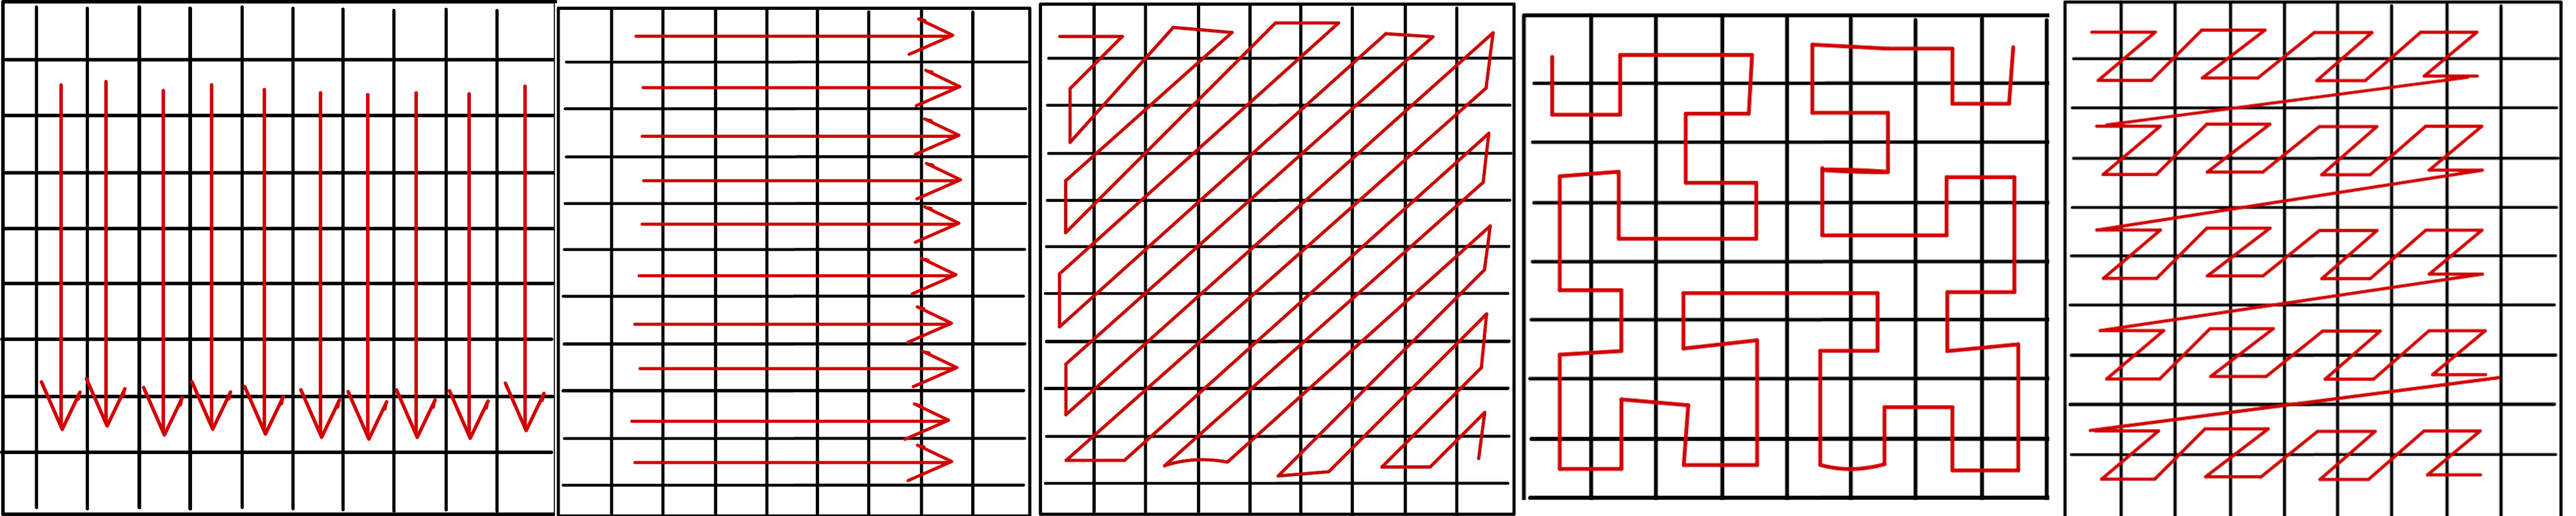
\includegraphics[scale=0.3]{images/scanning.png}
    \caption{Metody skenování obrazu}
    \label{fig:scanning}
\end{figure}

\section{Implementace}
V této sekci je popsána implementace adaptivního Huffmanova kódování a adaptivního skenování obrazu. 

Projekt je implementován v jazyce \texttt{c++} (standard \texttt{c++20}). V kódu je hojně využíváno template metaprogramování, díky čemuž je implementována i částečná podpora symbolů v jiné abecedě než \texttt{uint8\_t}. Tato podpora ovšem není plně funkční. Celá implementace se nachází v \texttt{namespace pf::kko}.

Ve zdrojových souborech je obsažena i implementace statického Huffmanova kódování, ale ta nebyla v zadání a proto zde není popsána.

\subsection{Adaptivní Huffmanovo kódování}
Společné struktury pro kódování a dekódování (práce se stromem) jsou umístěny v souboru \texttt{adaptive\_common.h}. Implementován je Viterr algoritmus, který je popsaný v předchozí sekci. Pro urychlení zpracování je použita cache k rychlejšímu dohledání uzlů podle symbolu - není nutné procházet celý strom. Data z disku jsou čtena za využití třídy \texttt{RawGrayscaleImageDataReader}. Pro strom je využita generická struktura \texttt{Tree<T>}, která implementuje binární strom. Pro zápis binárních dat existuje třída \texttt{BinaryEncoder}, která umožňuje serializaci dat, či přímý zápis bitových hodnot. 

Pro statické skenování jsou ve výstupních datech pouze data nutná k rekonstrukci stromu - kódy symbolů, či Huffmanův kód. Implementace je v souborech \texttt{adaptive\_encoding.h} a \texttt{adaptive\_decoding.h}.

Pro adaptivní skenování strom obsahuje hlavičku - 4B velikost obrázku, 2B velikost bloku. Dále každý blok obsahuje hlavičku, kdy jsou využity 3 bity pro uložení typu průchodu. 

\subsection{Adaptivní skenování}
Adaptivní skenování je implementováno třídou \texttt{AdaptiveImageScanner}. Třída přijímá v konstruktoru vstupní data, implementace konceptu \texttt{BlockScorer} pro hodnocení vhodnosti typu průchodu bloku a implementaci konceptu \texttt{Model} pro transformaci dat. Třída je implementována jako \texttt{range} objektů typu \texttt{Block}. Tento objekt reprezentuje vyhrazenou oblast ve vstupních datech, která je také \texttt{range}. Pomocí iterátorů lze procházet data bez závislosti na typu průchodu.

Pro hodnocení vhodnosti jsem implementoval 2 typy. Prvním je \texttt{SameNeighborsScorer}, který má tím vyšší skóre, čím vícekrát se po sobě opakují symboly v sekvenci. Druhým je \texttt{NeighborDifferenceScorer}, který hodnotí nejlépe ten typ průchodu, kdy je součet rozdílů všech sousedních dat nejnižší. Vhodnějším se ukázal být \texttt{SameNeighborsScorer}.

\subsection{Model}
Implementace modelů je limitována konceptem \texttt{Model}. Statický polymorfismus namísto dynamického byl zvolen kvůli výrazně lepší optimalizaci - např. \texttt{IdentityModel} je optimalizátorem naprosto odstraněn. \texttt{Model} vyžaduje 2 metody; \texttt{apply(T)} pro transformaci a \texttt{revert(T)} pro zpětnou transformaci.

\subsection{Použité knihovny}
Program využívá následující knihovny:
\begin{itemize}
    \item \texttt{libfmt} \footnote{\url{https://github.com/fmtlib/fmt}} -- formátování řetězců.
    \item \texttt{spdlog} \footnote{\url{https://github.com/gabime/spdlog}} -- logování.
    \item \texttt{argparse} \footnote{\url{https://github.com/p-ranav/argparse}} -- zpracování argumentů terminálu.
    \item \texttt{tl::expected} \footnote{\url{https://github.com/TartanLlama/expected}} -- implementace P0323R8 návrhu pro c++.
    \item \texttt{magic\_enum} \footnote{\url{https://github.com/Neargye/magic_enum}} -- statická reflexe pro enumy.
    \item \texttt{nanobench} \footnote{\url{https://github.com/martinus/nanobench}} -- benchmark.
\end{itemize}

\section{Vyhodnocení}

\subsection{Doba zpracování}
Měření bylo prováděno na serveru \texttt{merlin.fit.vutbr.cz} za pomocí knihovny \texttt{nanobench} - knihovna sama detekuje počet opakování pro zaručení stability výsledku.

Časy provádění kódování, uváděno v milisekundách(SH = static Huffman, AH = adaptive Huffman, AS = adaptive scanning):
\begin{table}[H]
\begin{tabular}{|r|l|l|l|l|l|l|}
\hline
\multicolumn{1}{|c|}{Soubor} & SH   & SH + model & AH     & AH + model & AH + AS & AH + AS + model \\ \hline
df1h.raw                     & 10.2 & 3.8        & 2760.3 & 18.2       & 2701.8  & 129.8           \\ \hline
df1hvx.raw                   & 5.1  & 3.1        & 369    & 430.7      & 379.6   & 49.3            \\ \hline
df1v.raw                     & 8.4  & 2.3        & 2100.8 & 20.7       & 2126.5  & 105.9           \\ \hline
hd01.raw                     & 4.9  & 5.1        & 1529.3 & 1374       & 1530.3  & 1483            \\ \hline
hd02.raw                     & 4.9  & 4.9        & 1486.5 & 1370.4     & 1490.8  & 1457.3          \\ \hline
hd07.raw                     & 12.3 & 5.8        & 1995.2 & 837.9      & 1934.7  & 1403.4          \\ \hline
hd08.raw                     & 5.1  & 5.5        & 537.8  & 873.9      & 545.7   & 952.716         \\ \hline
hd09.raw                     & 7.8  & 7.3        & 2227.6 & 1633.9     & 2222.3  & 1833.3          \\ \hline
hd12.raw                     & 6.9  & 6.2        & 2269.3 & 1235.1     & 2251.8  & 1677.3          \\ \hline
nk01.raw                     & 8.1  & 8.2        & 2171.6 & 2097.5     & 2166.9  & 2164.8          \\ \hline
\end{tabular}
\end{table}

Časy provádění dekódování, uváděno v milisekundách(SH = static Huffman, AH = adaptive Huffman, AS = adaptive scanning):
\begin{table}[H]
\begin{tabular}{|r|l|l|l|l|l|l|}
\hline
\multicolumn{1}{|c|}{Soubor} & SH  & SH + model & AH     & AH + model & AH + AS & AH + AS + model \\ \hline
df1h.raw                     & 4.1 & 1          & 2499.4 & 4.3        & 2443.8  & 57.8            \\ \hline
df1hvx.raw                   & 2.7 & 1.5        & 308.6  & 252        & 317     & 20.4            \\ \hline
df1v.raw                     & 4.2 & 1          & 1895   & 5.3        & 1935.3  & 46.5            \\ \hline
hd01.raw                     & 2.8 & 3          & 1192.2 & 1049.1     & 1212.8  & 1090.1          \\ \hline
hd02.raw                     & 2.8 & 3          & 1152.6 & 1040.7     & 1165.4  & 1066.3          \\ \hline
hd07.raw                     & 3.8 & 3.7        & 1673   & 744.4      & 1665.5  & 1231.3          \\ \hline
hd08.raw                     & 2.9 & 3.4        & 442.2  & 691        & 450.8   & 746.1           \\ \hline
hd09.raw                     & 4.9 & 5.1        & 2012.8 & 1489.4     & 2019.3  & 1587.5          \\ \hline
hd12.raw                     & 4.1 & 4          & 1968.3 & 1049.9     & 1963.6  & 1447.1          \\ \hline
nk01.raw                     & 5.4 & 5.6        & 2009.6 & 1932.6     & 2023    & 1846.2          \\ \hline
\end{tabular}
\end{table}

\subsection{Úroveň komprese}
Následující tabulka zobrazuje BPC (bits per character) pro jednotlivé typy komprese. (SH = static Huffman, AH = adaptive Huffman, AS = adaptive scanning).
\begin{table}[H]
\begin{tabular}{|r|l|l|l|l|l|l|}
\hline
\multicolumn{1}{|c|}{Soubor} & SH      & SH + model & AH      & AH + model & AH + AS & AH + AS + model \\ \hline
df1h.raw                     & 8.0079  & 1.00015    & 8.0127  & 1.00006    & 8.05975 & 1.24887         \\ \hline
df1hvx.raw                   & 4.58051 & 1.83655    & 4.58453 & 1.83804    & 4.63165 & 1.2012         \\ \hline
df1v.raw                     & 8.0079  & 1.00015    & 8.0127  & 1.00204    & 8.06021 & 1.24838         \\ \hline
hd01.raw                     & 3.88    & 3.40598    & 3.88501 & 3.40964    & 3.93225 & 3.55899          \\ \hline
hd02.raw                     & 3.70486 & 3.3324     & 3.71033 & 3.3367     & 3.75739 & 3.46353         \\ \hline
hd07.raw                     & 5.61279 & 3.85666    & 5.61771 & 3.85974    & 5.66519 & 4.18243         \\ \hline
hd08.raw                     & 4.23663 & 3.52628    & 4.24118 & 3.52911    & 4.28848 & 3.66193         \\ \hline
hd09.raw                     & 6.65979 & 4.68561    & 6.6669  & 4.68961    & 6.7142  & 5.05008         \\ \hline
hd12.raw                     & 6.20026 & 4.39148    & 6.20694 & 4.39508    & 6.25467 & 4.64194         \\ \hline
nk01.raw                     & 6.50854 & 6.06931    & 6.51367 & 6.07309    & 6.56082 & 5.83646         \\ \hline
\end{tabular}
\end{table}

Ne příliš dobré výsledky pro adaptivní skenování jsou pravděpodobně následek nevhodného hodnocení při výběru typu průchodu blokem obrazu.


\section{Překlad a použití programu}
Překlad je prováděn pomocí příkazu \texttt{make}. V defaultním režimu je vytvořen program \texttt{huff\_codec}, jehož použití je následující:

\begin{lstlisting}
Usage: huff_codec [options] 

Optional arguments:
-h --help       show this help message and exit
-c              Compress input file
-d              Decompress input file
-m              Activate model for preprocessing
-a              Adaptive scanning
-i              Path to input file[Required]
-o              Path to output file[Required]
--static        Static huffman
-w              Input image width[Required]

\end{lstlisting}

Další možností je \texttt{make bench}. Tímto příkazem je vytvořen program \texttt{bench}, který slouží k verifikaci algoritmu a výpočtu úrovně komprese či změření doby běhu algoritmů. Použití programu:

\begin{lstlisting}
Usage: bench [options] 

Optional arguments:
-h --help       show this help message and exit
-i              Path to folder with input files[Required]
--validate      Test encoding validity

\end{lstlisting}

\nocite{data_compr1}
\bibliographystyle{plain}
\begin{flushleft}
  \bibliography{references}
\end{flushleft}

\end{document}

